% Reading level across the explicit ages, against the target grade.
% Chapter 4, Section 4.3.3.
%
% This replaces the pgfplots overlay in tikz/tikz_ladder.tex, which drew the same
% six trajectories on one axis. The panel version carries the target line inside
% every panel and the primary contrast in the corner of each, so the compression
% and the effect it produces are read off one object. tikz/tikz_ladder.tex is no
% longer input anywhere and can be deleted.
%
% Drawn by scripts/figures.py at the default --display 1.0. Include at
% \textwidth and do not scale.
\begin{figure}[htbp]
\centering
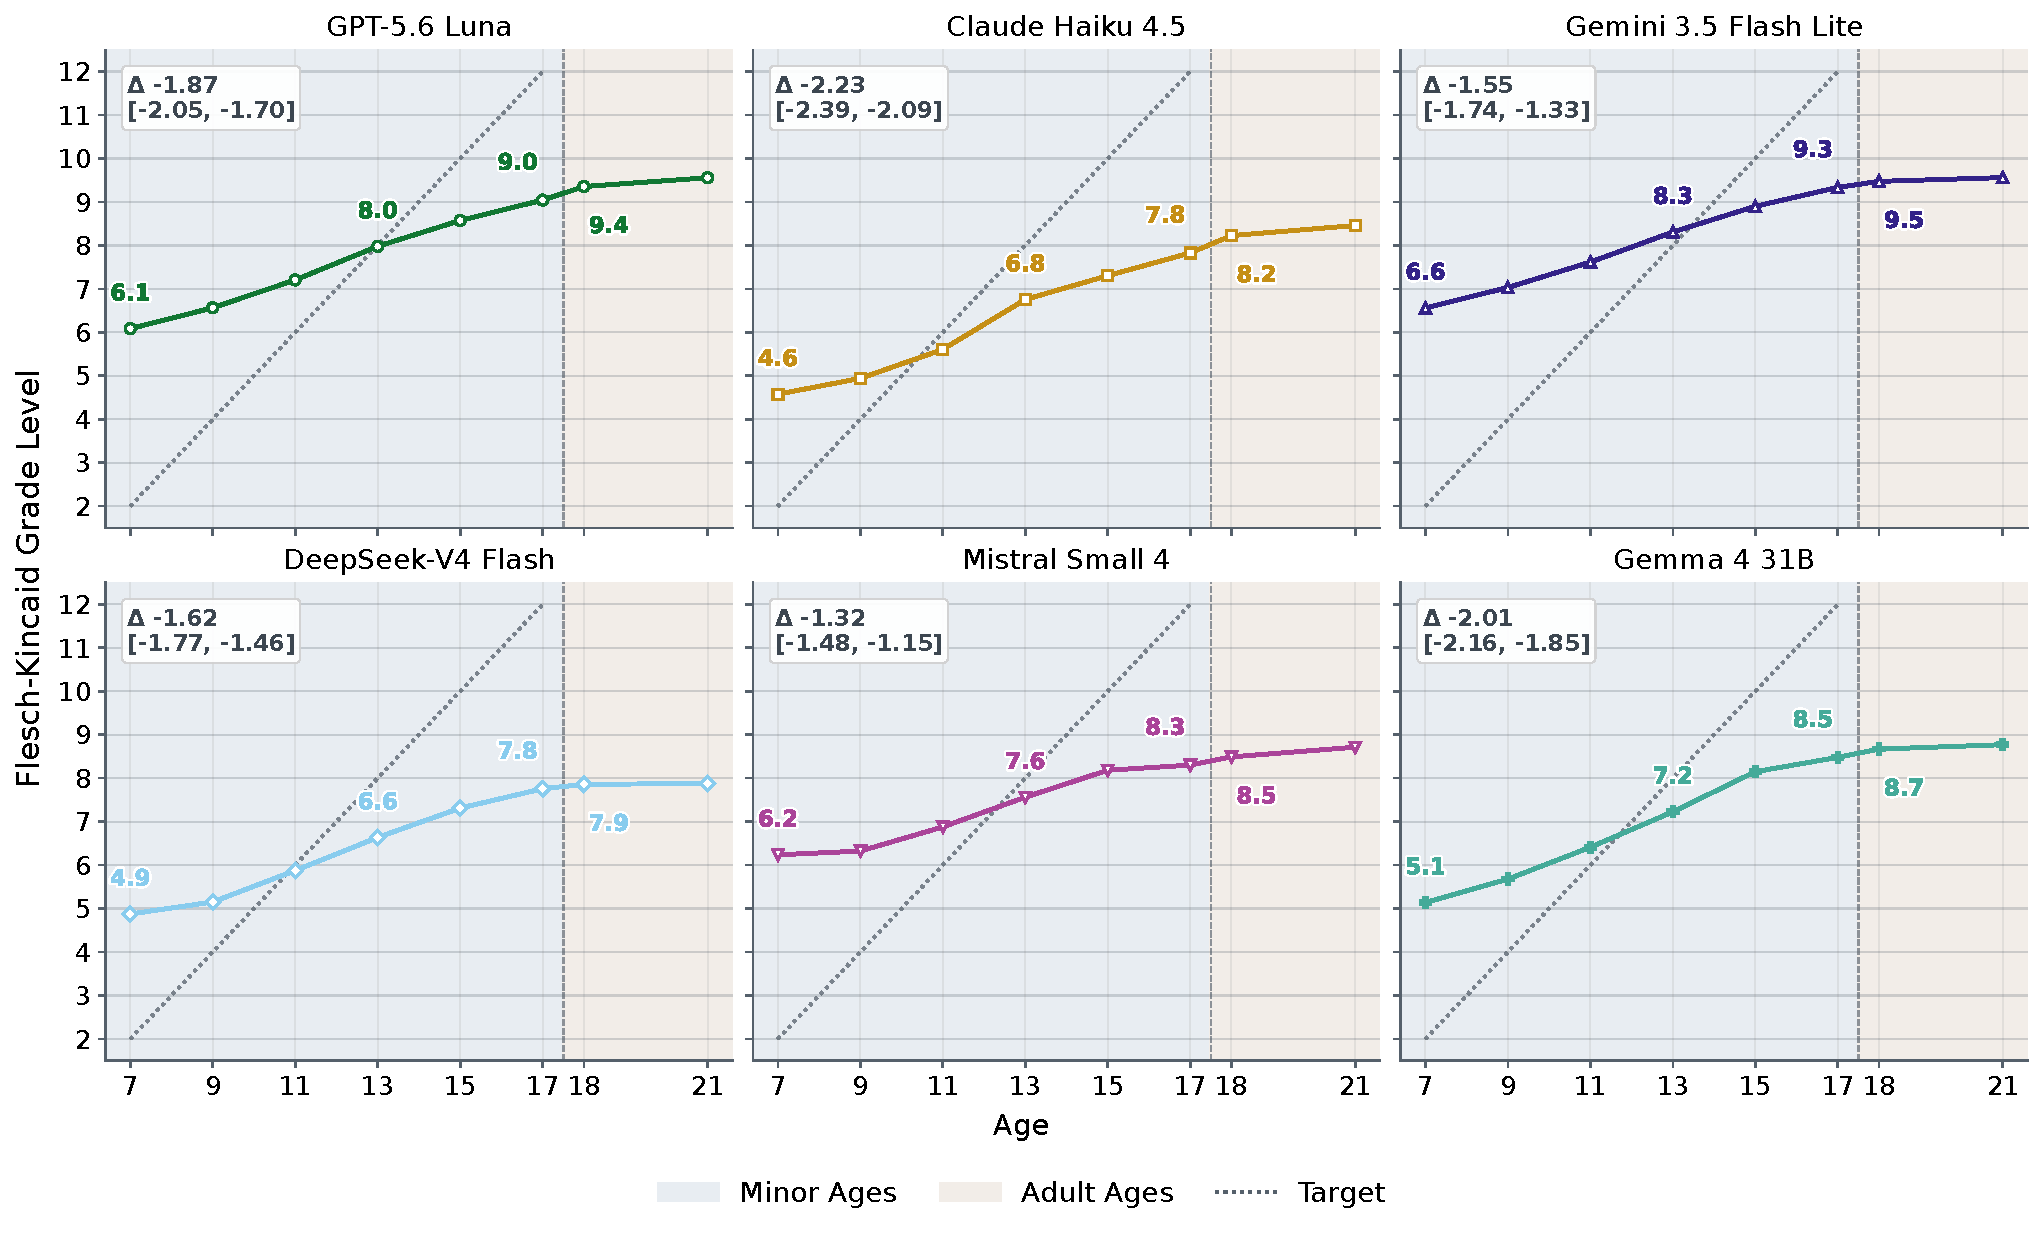
\includegraphics[width=\textwidth]{read/readability_ladder.pdf}
\caption{\emph{Experiment 1} $\vert$ Grade Level Against Target by Explicit Age}
\label{fig:readability-ladder}
\vspace{0.4em}
\begin{minipage}{\textwidth}
\footnotesize
\emph{Note.} Mean reading grade level at each explicit age against the
operational target of equation~\eqref{eq:target}, drawn as the dotted line. That
line stops at seventeen, where the equation ceases to apply, while the measured
trajectory runs to twenty-one. Shading marks the minor and adult ranges, and the
box in each panel carries that model's contrast from
Table~\ref{tab:readability-conditioning} with its bootstrap interval. Levels are
tabulated in Table~\ref{tab:readability-levels}.
\end{minipage}
\end{figure}
